% MIT License

% Copyright (c) 2022 Chiyuru

% Permission is hereby granted, free of charge, to any person obtaining a copy of this software and associated documentation files (the "Software"), 
% to deal in the Software without restriction, including without limitation the rights
% to use, copy, modify, merge, publish, distribute, sublicense, and/or sell
% copies of the Software, and to permit persons to whom the Software is
% furnished to do so, subject to the following conditions:

% The above copyright notice and this permission notice shall be included in all copies or subsubstantial portions of the Software.

% THE SOFTWARE IS PROVIDED "AS IS", WITHOUT WARRANTY OF ANY KIND, EXPRESS OR IMPLIED, INCLUDING BUT NOT LIMITED TO THE WARRANTIES OF MERCHANTABILITY,
% FITNESS FOR A PARTICULAR PURPOSE AND NONINFRINGEMENT. IN NO EVENT SHALL THE AUTHORS OR COPYRIGHT LASTERS BE LIABLE FOR ANY CLAIM, DAMAGES OR OTHER
% LIABILITY, WHETHER IN AN ACTION OF CONTRACT, TORT OR OTHERWISE, ARISING FROM,
% OUT OF OR IN CONNECTION WITH THE SOFTWARE OR THE USE OR OTHER DEALINGS IN THE SOFTWARE.

\documentclass[UTF8]{ctexart}

\usepackage{amsmath}
\usepackage{cases}
\usepackage{cite}
\usepackage{graphicx}
\usepackage[margin=1in]{geometry}
\usepackage{float}
\geometry{a4paper}
\usepackage{fancyhdr}
\usepackage{multirow}
\usepackage{listings}
\pagestyle{fancy}
\fancyhf{}


\title{ICS-lab5实验报告}
\author{孔浩宇 PB20000113}
\date{\today}
\pagenumbering{arabic}

\begin{document}

\fancyhead[L]{孔浩宇}
\fancyhead[C]{ICS-lab5实验报告}
\fancyfoot[C]{\thepage}

\maketitle
\tableofcontents
\newpage

\section{实验目的}
    实验的目的是展示中断驱动的输入/输出如何中断正在运行的程序,执行中断服务例程,
    并返回到被中断的程序,准确地从它离开的地方开始 (就像什么都没有发生一样)。

\section{实验原理}
    \subsection{实现带延迟的打印字符串}
    \begin{enumerate}
        \item [(1)]打印字符串ID
        \begin{lstlisting}[basicstyle=\ttfamily,language={[x86masm]Assembler}]
            LOOP    LEA R0, ID          ; 打印学号
                    PUTS             
        \end{lstlisting}

        \item [(2)]打印延迟 (防止速度过快)
        \begin{lstlisting}[basicstyle=\ttfamily,language={[x86masm]Assembler}]
                    AND R0, R0, #0
            LD      R0, COUNT
            REP     ADD R0, R0, #-1
                    BRp REP             ; 每两次打印之间进行延迟
                    BRnzp LOOP
            COUNT   .FILL #25000        ; 可调节         
        \end{lstlisting}
    \end{enumerate}

    \subsection{换行}
    用NEWLINE存储换行转义符的ASCII码,用R0存储并打印,实现换行
    \begin{lstlisting}[basicstyle=\ttfamily,language={[x86masm]Assembler}]
        LD  R0, NEWLINE     
        OUT                 ; 输出"\n",换行
    \end{lstlisting}

    \subsection{判断输入合法性}
    \begin{lstlisting}[basicstyle=\ttfamily,language={[x86masm]Assembler}]
        LD  R3, ASCIIZ
        ADD R0, R0, R3      ; n-'0'
        ADD R4, R0, #0      
        BRn ERROR           ; 非法输入
        LD  R3, ASCIIN     
        ADD R0, R5, R3      ; n-'9'
        BRp ERROR
        LEA R0, OUTPUT2 
        PUTS                ; 输入合法,输出反馈
        LD R0, NEWLINE
        OUT                 ; 输出"\n",换行
        ADD R0, R4, #0
        BR MAIN             ; 执行主程序
    \end{lstlisting}

    \subsection{实现汉诺塔公式}
    \begin{enumerate}
        \item [(1)]递归
        \begin{lstlisting}[basicstyle=\ttfamily,language={[x86masm]Assembler}]
            REC     ADD R0, R0, #-1             ; R0 = n-1
                    JSR HANOI                   ; R1 = H(n-1)
                    ADD R1, R1, R1              ; R1 = 2H(n-1)
                    ADD R1, R1, #1              ; R1 = 2H(n-1) + 1
        \end{lstlisting}
        \item [(2)]递归出口
        当n=0时,递归结束,底层函数返回0
        \begin{lstlisting}[basicstyle=\ttfamily,language={[x86masm]Assembler}]
            HANOI   ADD R6, R6, #-1
                    STR R7, R6, #0         ; R7入栈
                    ADD R6, R6, #-1
                    STR R0, R6, #0         ; R0入栈 (n)
                    ADD R6, R6, #-1
                    STR R2, R6, #0         ; R2入栈
                    AND R2, R0, #-1
                    BRzp REC        ; R0 = 0 -> R1 = 0 (递归出口)    
                    ADD R1, R0, #0         ; R1 = 0 is the answer
                    BRnzp DONE
        \end{lstlisting}
        \item [(3)]还原寄存器并返回
        \begin{lstlisting}[basicstyle=\ttfamily,language={[x86masm]Assembler}]
            DONE    LDR R2, R6, #0
            ADD R6, R6, #1
            LDR R0, R6, #0
            ADD R6, R6, #1
            LDR R7, R6, #0
            ADD R6, R6, #1
            RET
        \end{lstlisting}
    \end{enumerate}

    \subsection{打印三位十进制数}
    \begin{enumerate}
        \item [(1)]取R1最高位
        设最高位为第n位,则取NMAX为$- {10}^{n-1}$的补码,R0初始化为0的ASCII码,
        R1每次减去NMAX,非负则R0加1,最后R0即为此位数字的ASCII码
        \begin{lstlisting}[basicstyle=\ttfamily,language={[x86masm]Assembler}]
                LD  R0, ZERO
                LD  R2, NHUN
        LOOPH   ADD R1, R2, R1
                BRn ENDH
                ADD R0, R0, #1
                BRnzp LOOPH
        \end{lstlisting}
        \item [(2)]打印最高位
        \begin{lstlisting}[basicstyle=\ttfamily,language={[x86masm]Assembler}]
            ENDH    OUT                         ; 百位
        \end{lstlisting}
        \item [(3)]对后一位进行操作
        设最高位为第n位,则取PMAX为$- {10}^{n-1}$的补码,
        输出第n位结束后,R1为R1模PMAX再减去PMAX,加上PMAX后,R1最高位即为第n-1位,
        重复前两次操作即可
        \begin{lstlisting}[basicstyle=\ttfamily,language={[x86masm]Assembler}]
            LD R3, PMAX
            ADD R1, R1, R3
        \end{lstlisting}
    \end{enumerate}

\section{实验代码A:The user program}
\subsection{初始化}
\begin{enumerate}
    \item [(0)]标号
    \begin{lstlisting}[basicstyle=\ttfamily,language={[x86masm]Assembler}]
        COUNT   .FILL #25000        
        ID      .STRINGZ "PB20000113 "        
    \end{lstlisting}
\end{enumerate}
\subsection{打印学号}
    \begin{lstlisting}[basicstyle=\ttfamily,language={[x86masm]Assembler}]
        LOOP    LEA R0, ID      ; 打印学号
                PUTS
                AND R0, R0, #0
                LD  R0, COUNT
        REP     ADD R0, R0, #-1
                BRp REP         ; 每两次打印之间进行延迟
                BRnzp LOOP
    \end{lstlisting}
\section{实验代码B:The keyboard interrupt service routine}
\subsection{初始化}
\begin{enumerate}
    \item [(0)]标号
    \begin{lstlisting}[basicstyle=\ttfamily,language={[x86masm]Assembler}]
        ASCIIZ  .FILL   xFFD0               ; ASCII码0
        ASCIIN  .FILL   xFFC7               ; ASCII码9
        ZERO    .FILL   x0030               
        STACK   .FILL   x6000               ; 栈底
        NEWLINE .FILL   x000A               ; 换行转义符
        OUTPUT1 .STRINGZ " is not a decimal digit."     ; 输入非0-9时反馈
        OUTPUT2 .STRINGZ " is a decimal digit."         ; 输入0-9时反馈
        OUTPUT3 .STRINGZ "TOWER OF HANOI needs "
        OUTPUT4 .STRINGZ " moves."
        NHUN    .FILL   xFF9C
        PHUN    .FILL   x0064
        NTEN    .FILL   xFFF6
    \end{lstlisting}

    \item [(1)]初始化寄存器
    \begin{lstlisting}[basicstyle=\ttfamily,language={[x86masm]Assembler}]
        ADD R6, R6, #-1
        STR R0, R6, #0
    \end{lstlisting}
\end{enumerate}

\subsection{检查输入合法性}
    \begin{lstlisting}[basicstyle=\ttfamily,language={[x86masm]Assembler}]
            GETC                ;从键盘读入n (ASCII码)
            OUT
            ADD R5, R0, #0
            LD  R3, ASCIIZ
            ADD R0, R0, R3      ; n-'0'
            ADD R4, R0, #0      
            BRn ERROR           ; 非法输入
            LD  R3, ASCIIN     
            ADD R0, R5, R3      ; n-'9'
            BRp ERROR
            LEA R0, OUTPUT2 
            PUTS                ; 输入合法,输出反馈
            LD R0, NEWLINE
            OUT                 ; 输出"\n",换行
            ADD R0, R4, #0
            BR MAIN
    ERROR   LEA R0, OUTPUT1
            PUTS                ; 非0-9,输出反馈
    FINISH  LD  R0, NEWLINE
            OUT
            RTI
    \end{lstlisting}

\subsection{汉诺塔子程序}
\begin{lstlisting}[basicstyle=\ttfamily,language={[x86masm]Assembler}]
HANOI   ADD R6, R6, #-1
        STR R7, R6, #0              ; R7入栈
        ADD R6, R6, #-1
        STR R0, R6, #0              ; R0入栈 (n)
        ADD R6, R6, #-1
        STR R2, R6, #0              ; R2入栈
        AND R2, R0, #-1
        BRzp REC                    ; R0 = 0 时,R1 = 0 (递归出口)    
        ADD R1, R0, #0              ; R1 = 0 is the answer
        BRnzp DONE

REC     ADD R0, R0, #-1             ; R0 = n-1
        JSR HANOI                   ; R1 = H(n-1)
        ADD R1, R1, R1              ; R1 = 2H(n-1)
        ADD R1, R1, #1              ; R1 = 2H(n-1) + 1
DONE    LDR R2, R6, #0
        ADD R6, R6, #1
        LDR R0, R6, #0
        ADD R6, R6, #1
        LDR R7, R6, #0
        ADD R6, R6, #1
        RET
\end{lstlisting}

\subsection{打印汉诺塔递归结果}
\begin{lstlisting}[basicstyle=\ttfamily,language={[x86masm]Assembler}]
        JSR HANOI
        LEA R0, OUTPUT3
        PUTS
        LD  R0, ZERO
        LD  R2, NHUN
LOOPH   ADD R1, R2, R1
        BRn ENDH
        ADD R0, R0, #1
        BRnzp LOOPH
ENDH    OUT                         ; 百位
        LD R3, PHUN
        ADD R1, R1, R3
        LD R0, ZERO
        LD R2, NTEN
LOOPS   ADD R1, R2, R1
        BRn ENDS
        ADD R0, R0, #1
        BRnzp LOOPS
ENDS    OUT                         ; 十位
        ADD R1, R1, #10
        LD R0, ZERO
        ADD R0, R0, R1
        OUT                         ; 个位
        LEA R0, OUTPUT4
        PUTS
        HALT
\end{lstlisting}


\clearpage
\section{代码}    
\begin{lstlisting}[basicstyle=\ttfamily,language={[x86masm]Assembler}]
    .ORIG x800
    ; (1) Initialize interrupt vector table.
    LD R0, VEC
    LD R1, ISR
    STR R1, R0, #0

    ; (2) Set bit 14 of KBSR.
    LDI R0, KBSR
    LD R1, MASK
    NOT R1, R1
    AND R0, R0, R1
    NOT R1, R1
    ADD R0, R0, R1
    STI R0, KBSR

    ; (3) Set up system stack to enter user space.
    LD R0, PSR
    ADD R6, R6, #-1
    STR R0, R6, #0
    LD R0, PC
    ADD R6, R6, #-1
    STR R0, R6, #0
    ; Enter user space.
    RTI
VEC     .FILL   x0180
ISR     .FILL   x1000
KBSR    .FILL   xFE00
MASK    .FILL   x4000
PSR     .FILL   x8002
PC      .FILL   x3000
    .END

    .ORIG x3000
    ; *** Begin user program code here ***
LOOP    LEA R0, ID      ; 打印学号
        PUTS
        AND R0, R0, #0
        LD  R0, COUNT
REP     ADD R0, R0, #-1
        BRp REP         ; 每两次打印之间进行延迟
        BRnzp LOOP
COUNT   .FILL #25000        
ID      .STRINGZ "PB20000113 "        
    ; *** End user program code here ***
    .END

    .ORIG x3FFF
    ; *** Begin honoi data here ***
HONOI_N .FILL xFFFF
    ; *** End honoi data here ***
    .END

    .ORIG x1000
    ; *** Begin interrupt service routine code here ***
        LD  R6, STACK       ; 压栈
        LD  R0, NEWLINE     
        OUT                 ; 输出"\n",换行
        GETC                ;从键盘读入n (ASCII码)
        OUT
        ADD R5, R0, #0
        LD  R3, ASCIIZ
        ADD R0, R0, R3      ; n-'0'
        ADD R4, R0, #0      
        BRn ERROR           ; 非法输入
        LD  R3, ASCIIN     
        ADD R0, R5, R3      ; n-'9'
        BRp ERROR
        LEA R0, OUTPUT2 
        PUTS                ; 输入合法,输出反馈
        LD R0, NEWLINE
        OUT                 ; 输出"\n",换行
        ADD R0, R4, #0
        BR MAIN
ERROR   LEA R0, OUTPUT1
        PUTS                ; 非0-9,输出反馈
FINISH  LD  R0, NEWLINE
        OUT
        RTI
   
MAIN    ADD R6, R6, #-1
        STR R0, R6, #0
        JSR HANOI
        LEA R0, OUTPUT3
        PUTS
        LD  R0, ZERO
        LD  R2, NHUN
LOOPH   ADD R1, R2, R1
        BRn ENDH
        ADD R0, R0, #1
        BRnzp LOOPH
ENDH    OUT                         ; 百位
        LD R3, PHUN
        ADD R1, R1, R3
        LD R0, ZERO
        LD R2, NTEN
LOOPS   ADD R1, R2, R1
        BRn ENDS
        ADD R0, R0, #1
        BRnzp LOOPS
ENDS    OUT                         ; 十位
        ADD R1, R1, #10
        LD R0, ZERO
        ADD R0, R0, R1
        OUT                         ; 个位
        LEA R0, OUTPUT4
        PUTS
        HALT

HANOI   ADD R6, R6, #-1
        STR R7, R6, #0              ; R7入栈
        ADD R6, R6, #-1
        STR R0, R6, #0              ; R0入栈 (n)
        ADD R6, R6, #-1
        STR R2, R6, #0              ; R2入栈
        AND R2, R0, #-1
        BRzp REC                    ; R0 = 0 时,R1 = 0 (递归出口)    
        ADD R1, R0, #0              ; R1 = 0 is the answer
        BRnzp DONE

REC     ADD R0, R0, #-1             ; R0 = n-1
        JSR HANOI                   ; R1 = H(n-1)
        ADD R1, R1, R1              ; R1 = 2H(n-1)
        ADD R1, R1, #1              ; R1 = 2H(n-1) + 1
DONE    LDR R2, R6, #0
        ADD R6, R6, #1
        LDR R0, R6, #0
        ADD R6, R6, #1
        LDR R7, R6, #0
        ADD R6, R6, #1
        RET
ASCIIZ  .FILL   xFFD0               ; ASCII码0补码
ASCIIN  .FILL   xFFC7               ; ASCII码9补码
ZERO    .FILL   x0030               
STACK   .FILL   x6000               ; 栈底
NEWLINE .FILL   x000A               ; 换行转义符
OUTPUT1 .STRINGZ " is not a decimal digit."     ; 输入非0-9时反馈
OUTPUT2 .STRINGZ " is a decimal digit."         ; 输入0-9时反馈
OUTPUT3 .STRINGZ "TOWER OF HANOI needs "
OUTPUT4 .STRINGZ " moves."
NHUN    .FILL   xFF9C               ; -100
PHUN    .FILL   x0064               ; +100
NTEN    .FILL   xFFF6               ; -10
    ; *** End interrupt service routine code here ***
    .END
\end{lstlisting}

\clearpage
\section{实验结果}
\subsection{十进制输入}
    \begin{figure*}[htbp]
        \centering
        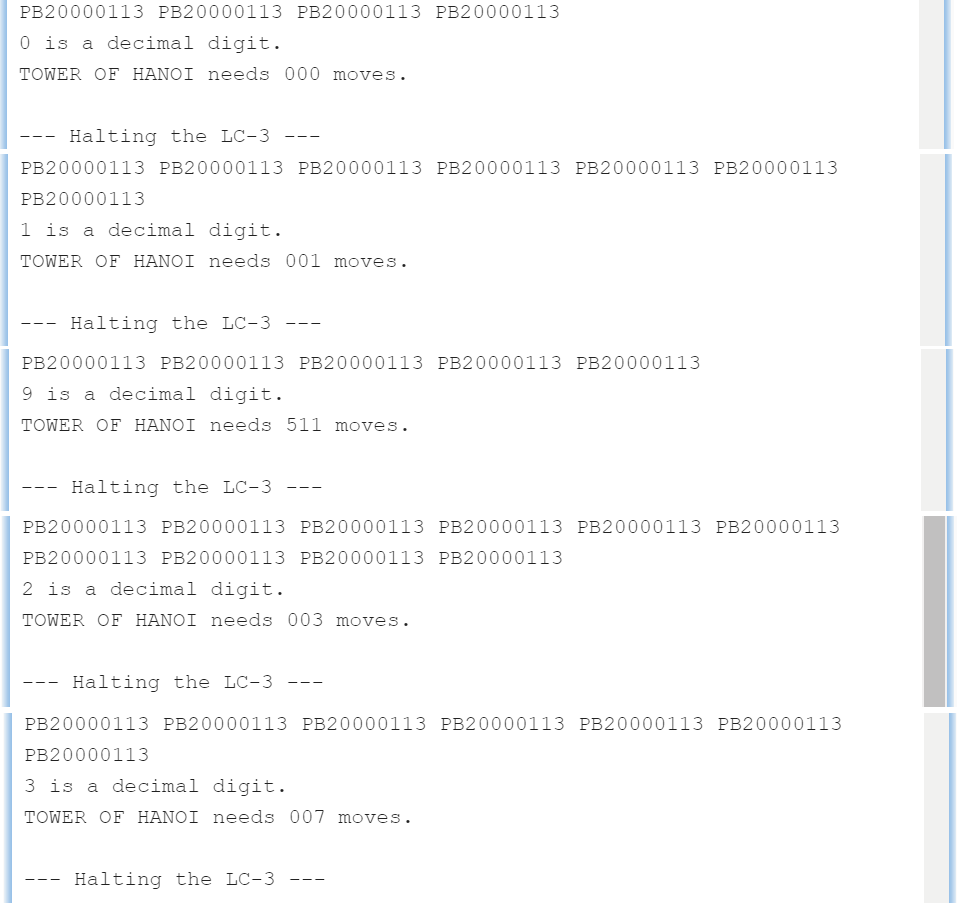
\includegraphics[scale=0.6]{de.png}
    \end{figure*}
\subsection{非法输入}
    \begin{figure*}[htbp]
        \centering
        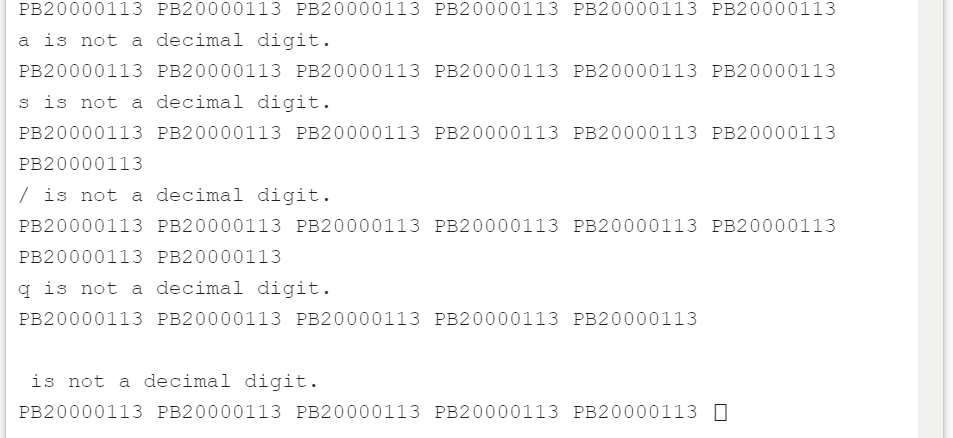
\includegraphics[scale=0.6]{r.png}
    \end{figure*}
\end{document}
\begin{lstlisting}[basicstyle=\ttfamily,language={[x86masm]Assembler}]

\end{lstlisting}